\documentclass[11pt]{scrartcl}

% own geometry
\usepackage[a4paper, left=3cm, right=3cm]{geometry}

\usepackage[ngerman]{babel} 
\usepackage[utf8]{inputenc} 
\usepackage[T1]{fontenc}
\usepackage{graphicx}
\usepackage{color}
\usepackage{xcolor}

% setup of source code listings
\usepackage{listings}
\usepackage{courier}
\usepackage{caption}
\lstset{
	basicstyle=\footnotesize\ttfamily,	% default font
	numbers=left,						% line numbers placement
	numberstyle=\tiny,					% line numbers style
	%stepnumber=2,						% line number padding
	numbersep=5pt,						% padding between line numbers and code
	tabsize=2,							% 
	extendedchars=true,         
	breaklines=true,						% line breaks 
	keywordstyle=\color{red},
	frame=b,
	stringstyle=\color{white}\ttfamily,	% color of strings in code
	showspaces=false,					% visualize spaces
    showtabs=false,						% visualize tabs
    xleftmargin=17pt,
	framexleftmargin=17pt,
	framexrightmargin=5pt,
	framexbottommargin=4pt,
	showstringspaces=false				% visualize spaces in strings        
 }
 
 \lstloadlanguages{% Check docs for further languages ...
         C,
         C++
 }

%\captionsetup[lstlisting]{singlelinecheck=false, labelfont={blue}, textfont={blue}}

\DeclareCaptionFont{white}{\color{white}}
\DeclareCaptionFormat{listing}{\colorbox{gray}{\parbox{\textwidth}{#1#2#3}}}
\captionsetup[lstlisting]{format=listing,labelfont=white,textfont=white}

% layout the box
%\DeclareCaptionFormat{listing}{\colorbox[rgb]{0.43, 0.35, 0.35 {\parbox{\textwidth}{\hspace{15pt}#1#2#3}}}

% layout the caption ontop of code
\captionsetup[lstlisting]{format=listing,labelfont=white,textfont=white, singlelinecheck=false, margin=0pt, font={bf,footnotesize}}

% Document begins now
\begin{document}

\author{ Martin Helmich, Oliver Erxleben \\ \\ Hochschule Osnabr"uck \\
Ingenieurswissenschaften und Informatik \\ Informatik - Mobile und Verteilte Anwendungen
\\ \\ martin.helmich@hs-osnabrueck.de \\ oliver.erxleben@hs-osnabrueck.de }

\title{
\includegraphics[scale=0.75,keepaspectratio]{img/hs_os.png}\linebreak \linebreak
OpenMP [Working DRAFT]}

\maketitle
\thispagestyle{empty}
\tableofcontents

\pagebreak
\pagestyle{plain}
\setcounter{page}{1}
\section{OpenMP} Open Multi-Processing (kurz: OpenMP) ist eine Programmierschnittstelle
f"ur die Sprachen C/C++ und Fortran, welche seit 1997 von unterschiedlichen Hardware- und Compilerherstellern entwickelt wird. Ziel von OpenMP, welches mittlerweile den
Versionsstand 3.1 erreicht hat, ist es ein portables und zugleich paralleles
Programmiermodell f"ur Shared-Memory-Architekturen\footnote{Shared-Memory-Architektur: } zur Verf"ugung zu stellen. Es setzt sich aus Compilerdirektiven, Bibliotheksfunktionen und Umgebungsvariablen zusammen. Anders als viele alternative Ansätze zur Parallelisierung von Programmen sind nur wenige Änderungen an sequenziellen Programmen notwendig um parallele Abläufe zu implementieren. Auch die Lesbarkeit des parallelisierten Quelltextes wird im Vergleich zu anderen alternativen Ansätzen stark verbessert. \textit{(Vgl. \cite{omp08} Kapitel 1: Einf"uhrung)} \\ Ein weiteres Plus f"ur den Einsatz von OpenMP ist die weite Verbreitung von Multi-Core-Rechnern und die Implementierung in vielen verbreiteten Compilern. So ist OpenMP im GCC seit der Version 4.2, im Visual Studio C/C++ Compiler seit der Version 2005 oder im Intel C/C++-Compiler seit Version 8 verf"ugbar. Compiler die keine OpenMP-Unterst"utzung bieten, ignorieren aufgrund der Pragma-Compilerdirektiven die Ausf"uhrung als parallelisierte OpenMP-Implementierung, was zu einer guten Portabilität f"uhrt. \\
Ursprünglich wurde OpenMP für den Bereich High Performance Computing entwickelt, wo Programmcode meist viele Schleifen enthält. Demnach ist die Parallelisierung von Schleifen die Hauptaufgabe von OpenMP und die meisten Vorteile können an dieser Stelle von OpenMP aufgezeigt werden. 
% TODO: Beispiel einfügen??

\subsection{Merkmale von OpenMP}

Mit OpenMP wird ein hoher \textbf{Abstraktionsgrad} erreicht, da Threads nicht durch einen Programmierer initialisiert, gestartet oder beenden werden m"ussen. Wie bereits in der Einf"uhrung erwähnt, beitet OpenMP eine gute \textbf{Portabilität} des Programms an, zum einen ist OpenMP in vielen Mainstream-Compilern implementiert, zum anderen können Compiler ohne OpenMP-Unterst"utzung das Programm ohne Veränderung kompilieren, da die Compilerdirektiven durch Pragmas eingesetzt und ignoriert werden können. Auch bleibt der sequenzielle Programmcode vollständig erhalten, wenn nicht mittels OpenMP kompiliert wird. Der Quelltext kann somit \textbf{Schrittweise parallelisiert} werden. 

\subsection{Ausführungsmodell} Die parallele Ausf"uhrung erfolgt durch Threads auf dem
Fork-/Join\footnote{Fork/Join:}-Ausf"uhrungsmodell. Zu Beginn eines Programms ist nur ein Thread aktiv, der sog. \textit{Master Thread}. Sobald bei der Programmausf"uhrung die Direktive \textit{\#pragma omp parallel \{ ... \} } erreicht wird, gabelt sich die
Ausf"uhrung in Threads auf. Die erstellten Threads werden als \textit{team of threads}
bezeichnet\footnote{Die Implementierung von OpenMP entscheidet "uber die Art der Threads die erstellt werden. Es könnten Threds auf Basis der PThreads-Bibliothek oder aber auch als vollwertige Shared-Memory-Prozesse umgesetzt sein.}. F"ur OpenMP, bzw. der Entwicklung mit OpenMP stellen Threads einen Kontrollfluss mit gemeinsamen Adressraum dar. \\ 
Die schließende geschweifte Klammer ist zudem ein Synchronisationspunkt, andem das team of threads auf alle Teammitglieder wartet. Die Abbildung \ref{Join-Fork-Modell} stellt einen möglichen Ablauf mit OpenMP dar.

\begin{figure}[h!]
\centering
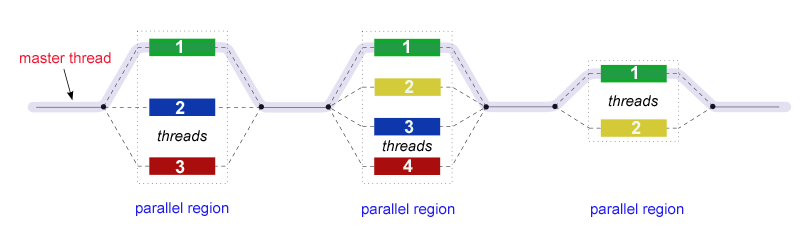
\includegraphics[width=1.0\textwidth]{img/fork_join.png}
\label{Join-Fork-Modell}
\caption{Fork-Join-Prinzip}
\protect{\textit{Entnommen aus OpenMP Tutorial} (siehe \cite{openmptut})}
\end{figure}

\subsection{Parallelisierung von Schleifen} 
Nach der Klassifikation von Flynn kann OpenMP als Single Programm Multiple Data (SPMD) beschrieben werden. Demnach führt jeder Thread der gestartet wurde den Schleifenblock aus. Dabei hat jeder Thread seine eigene Iteration und Teilmenge von Daten.\textit{(Vgl. siehe \cite{omp08}, Kapitel 3.1: Parallelität auf Schleifenebene)} \\
Ein team of threads wird mittels \textit{\#pragma omp parallel} gestartet. Zur Veranschaulichung sei das Listing \ref{parallelExample} gegeben. 

\lstinputlisting[caption= pragma omp parallel - Beispiel, label=parallelExample]{../src/1_3_example/parallel.c}
Die For-Schleife in Zeile 8 wird von allen vom System zur Verfügung stehenden Threads ausgeführt. Allerdings teilen sich die Threads nicht die Arbeit, sondern jeder Thread führt die Schleife komplett für sich aus. Um eine Schleife parallel auszuführen, muss über eine weitere Direktive, wie in Listing \ref{parallelForExample} zu sehen, eingefügt werden. 

\lstinputlisting[caption= pragma omp parallel for - Beispiel, label=parallelForExample]{../src/1_3_example/parallelfor.c} \\

In diesem Beispiel wird der zu parallelisierende Bereich eine Variable \textit{tid}, die threadId, übergeben. Jeder Thread erhält diese Variable, die nicht gemeinsam genutzt werden kann (private). 

\subsection{Synchronisation} 

\subsection{Abschnitte und Aufgaben}

\pagebreak % first part ends

\section{Vergleich mit TBB und anderen?!}

Text Text Text Text Text Text Text Text Text Text Text Text Text Text Text Text Text Text
Text Text Text Text Text Text Text Text Text Text Text Text Text Text Text Text Text Text
Text Text Text Text Text Text Text Text Text Text Text Text Text Text Text Text Text Text
Text Text.

\subsection{Unterkapitel"uberschrift}

Text Text Text Text Text Text Text Text Text Text Text Text Text Text Text Text Text Text
Text Text Text Text Text Text Text Text Text Text Text Text Text Text Text Text Text Text
Text Text.

%\begin{figure}[htb] %  \begin{center} %    \includegraphics[width=2cm]{gilogo} %   
%\caption{\label{logo}Beschreibung der Abbildung} %  \end{center} %\end{figure}

Text Text Text Text Text Text Text Text Text Text Text Text Text Text Text Text Text Text
Text Text Text Text Text Text Text Text Text Text Text Text Text Text Text Text Text Text
Text Text.

Text mit Fußnote.\footnote{Dies ist eine Fußnote. Text Text Text Text Text Text Text Text
Text Text Text Text Text Text Text Text Text Text Text.} Text \cite{Ez99,ABC01} Text Text
Text Text Text Text Text Text Text Text Text Text Text Text Text Text Text Text Text Text
Text Text Text Text Text Text Text Text  Text Text Text Text Text Text Text Text Text Text
Text Text Text Text Text Text Text Text Text Text Text Text Text Text Text Text Text Text
Text Text Text Text Text Text Text Text Text Text Text Text Text.

\pagebreak
\thispagestyle{empty}
\listoffigures

\listoftables

\lstlistoflistings

\begin{thebibliography}{3}
	\bibitem{omp08} S. Hoffmann, R. Lienhart: OpenMP - Eine Einf{\"u}hrung in die parallele Programmierung in C/C++
	
	\bibitem{openmptut} Blaise Barney, Lawrence Livermore National Laboratory: OpenMP Tutorial \\ https://computing.llnl.gov/tutorials/openMP/ \\ \textit{abgerufen am 24.11.2012}
\end{thebibliography}

\end{document}